%!TEX root=ast2016.tex

\begin{figure*}[t]
  \vspace*{-.25em}
  \centering
  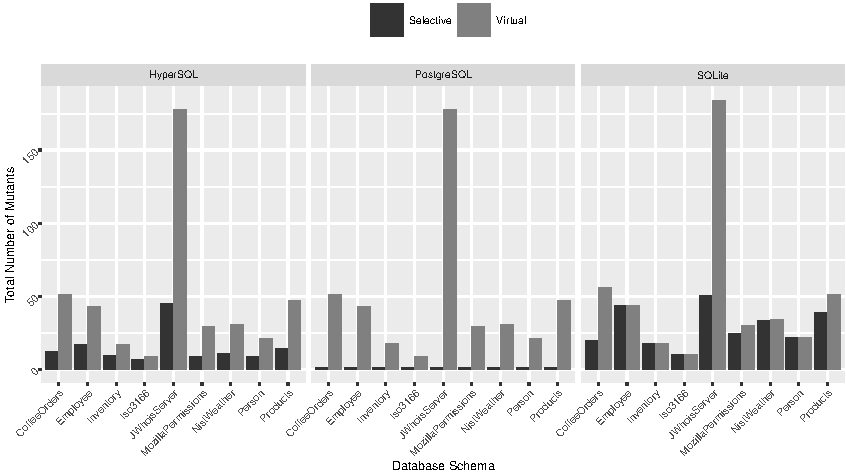
\includegraphics[scale=1.0]{graphics/graphic_barplot_schema_mutantcount_vm_tcm.pdf}
  % \vspace*{-.5em}
  \caption{Bar plot of the mutant count for both the selective and virtual mutation analysis techniques.}
  \label{fig:graphic_barplot_schema_mutantcount_vm_tcm}

  {\small \justifying{ \noindent In this plot the height of the bar corresponds to the number of mutants subject to
      analysis by the selective and virtual methods, reported for all of the schemas and the three DBMSs. Since
      the selective technique employs randomness to pick mutants that can be run within a specified time limit,
      the height of a dark grey bar is the average across a total of thirty runs; virtual mutation is deterministic and
  thus the height of the light grey bar is a direct count. } \par}

  \vspace*{-1em}

\end{figure*}
